% ============================================================================
%  dados.tex — tudo que muda de uma proposta para outra
%
%  O esqueleto (apresentacao.tex) só lê estes comandos. Quando a PACEcalculator
%  passar a gerar a apresentação, é este arquivo que ela escreve — e mais a
%  pasta figuras/. Nada aqui é lógica: são valores já formatados em pt-BR,
%  com o cifrão já escapado (R\$) e o percentual já escapado (\%).
%
%  Os valores abaixo são os da proposta Shaped, de 10/09/2026, e servem de
%  exemplo do formato esperado de cada campo.
% ============================================================================

% ---- Identificação --------------------------------------------------------
\newcommand{\cliente}{Shaped}
\newcommand{\dataproposta}{10 de setembro de 2026}
\newcommand{\tituloproposta}{Proposta Final de Inteligência Energética}
\newcommand{\responsavel}{Hans Wagner Glück}
\newcommand{\responsavelregistro}{CREA RS 248388}
\newcommand{\responsavelcredenciais}{Engenheiro Eletricista -- MSc Engenharia Nuclear -- Instituto Militar de Engenharia (IME)}
\renewcommand{\rodapereferencia}{Proposta para \cliente}

% ---- Sistema fotovoltaico (slide "Geração Fotovoltaica") ------------------
\newcommand{\subtitulosistema}{Melhor oportunidade para retorno financeiro e atendimento do projeto arquitetônico}
\newcommand{\potenciaprojeto}{26,32 kWp}
\newcommand{\potenciamodulo}{585 Wp}
\newcommand{\qtdmodulos}{45}
\newcommand{\potenciainversor}{7,5 kW SP \& 2 kW Micro}
\newcommand{\qtdinversores}{1 + 7}
\newcommand{\areaocupada}{140 m\textsuperscript{2}}
\newcommand{\producaoanual}{42,26 MWh}
\newcommand{\bess}{1 x 5 kWh}
% A foto aérea com os módulos sobrepostos. É a única figura por proposta.
\newcommand{\fototelhado}{figuras/foto_telhado.png}

% ---- Compra à vista ---------------------------------------------------------
\newcommand{\solucao}{Telhado}
\newcommand{\geracaoanual}{42.260 kWh}
\newcommand{\investimento}{R\$ 159.800,00}
\newcommand{\economiaanual}{R\$ 59.299,80 + Tarifa}
\newcommand{\rotulopayback}{Payback descontado}
\newcommand{\payback}{32 meses}
\newcommand{\gerenciamentomensal}{R\$ 40,00/mês}
\newcommand{\seguromensal}{R\$ 40,00/mês}
\newcommand{\rotulotir}{Retorno anual (TIR 25 anos)}
\newcommand{\tir}{37\% a.a.}

% ---- Compra financiada ------------------------------------------------------
\newcommand{\investimentocurto}{R\$ 159.800}
\newcommand{\economiamensal}{R\$ 4.900 + Tarifa}
\newcommand{\mensalidadefinanciada}{R\$ 5.056 + IPCA}
\newcommand{\segurofinanciado}{R\$ 40}
\newcommand{\gerenciamentofinanciado}{R\$ 40}
\newcommand{\prazofinanciamento}{5 anos}
\newcommand{\carenciafinanciamento}{3 meses}
\newcommand{\validadeproposta}{15 dias}

% ---- Leasing (as a service) -------------------------------------------------
\newcommand{\mensalidadeleasing}{R\$ 4.212 + Tarifa}
\newcommand{\prazoleasing}{10 anos}
\newcommand{\carencialeasing}{3 meses}

% ---- Desembolso mensal (uma linha por cenário) ------------------------------
% \linhadesembolso{cenário}{investimento}{mensalidade}{custo mensal}{economia mensal}{saldo mensal}
% Envolva em \positivo{} ou \negativo{} os saldos que devem sair no semáforo.
\newcommand{\linhasdesembolso}{%
  \linhadesembolso{À vista}{R\$ 159.800}{R\$ --}{R\$ 80,00}{R\$ 4.900,00}{\positivo{R\$ 4.820,00}}
  \linhadesembolso{Financiado}{R\$ --}{R\$ 5.055,36}{R\$ 80,00}{R\$ 4.900,00}{\negativo{--R\$ 235,36}}
  \linhadesembolso{As a Service}{R\$ --}{R\$ 4.212,00}{--}{R\$ 4.900,00}{\positivo{R\$ 688,00}}
}

% ---- Fluxo de caixa acumulado -----------------------------------------------
% Duas representações do mesmo número: a tabela recebe o texto já formatado,
% o gráfico recebe o valor cru. Quem escreve este arquivo cuida de os dois
% baterem.
% \linhafluxo{ano}{à vista}{financiado}{as a service}
\newcommand{\linhasfluxo}{%
  \linhafluxo{1}{\negativo{--R\$ 101.960,00}}{\negativo{--R\$ 2.824,26}}{\positivo{R\$ 8.256,00}}
  \linhafluxo{2}{\negativo{--R\$ 44.120,00}}{\negativo{--R\$ 5.648,52}}{\positivo{R\$ 16.512,00}}
  \linhafluxo{3}{\positivo{R\$ 13.720,00}}{\negativo{--R\$ 8.472,79}}{\positivo{R\$ 24.768,00}}
  \linhafluxo{5}{\positivo{R\$ 129.400,00}}{\negativo{--R\$ 14.121,31}}{\positivo{R\$ 41.280,00}}
  \linhafluxo{10}{\positivo{\bfseries R\$ 418.600,00}}{\positivo{\bfseries R\$ 275.078,69}}{\positivo{\bfseries R\$ 82.560,00}}
  \linhafluxo{25}{\positivo{R\$ 1.286.200,00}}{\positivo{R\$ 1.142.678,69}}{\positivo{R\$ 964.560,00}}
}
% Os mesmos anos, na mesma ordem, para o eixo x do gráfico.
\newcommand{\fluxoanos}{1,2,3,5,10,25}
% A linha do zero vai do primeiro ao último ano.
\newcommand{\fluxozero}{(1,0) (25,0)}
% A ressalva embaixo das duas tabelas financeiras.
\newcommand{\notafluxo}{Números a valor presente. Considerando as projeções, os resultados devem ser ainda melhores.}
\newcommand{\fluxoavista}{(1,-101960) (2,-44120) (3,13720) (5,129400) (10,418600) (25,1286200)}
\newcommand{\fluxofinanciado}{(1,-2824.26) (2,-5648.52) (3,-8472.79) (5,-14121.31) (10,275078.69) (25,1142678.69)}
\newcommand{\fluxoservico}{(1,8256) (2,16512) (3,24768) (5,41280) (10,82560) (25,964560)}

% ---- Lista de equipamentos (anexo) ------------------------------------------
% \linhaequipamento{equipamento}{marca}{quantidade}{potência}{garantia}
% A marca pode ser texto ou uma imagem: \includegraphics[height=0.2cm]{...}
\newcommand{\linhasequipamentos}{%
  \linhaequipamento{Inversor}{\raisebox{-0.2\height}{
\includegraphics[height=0.2cm]{estaticas/marca-goodwe.png}}}{--}{Diversos}{10 anos}
  \linhaequipamento{Módulo}{DAH / Longi}{--}{615 Wp}{10 / 20 anos}
  \linhaequipamento{Estrutura}{Carport}{--}{--}{20 anos}
}
% As fotos que ilustram a lista (até três, lado a lado).
\newcommand{\fotosequipamentos}{%
  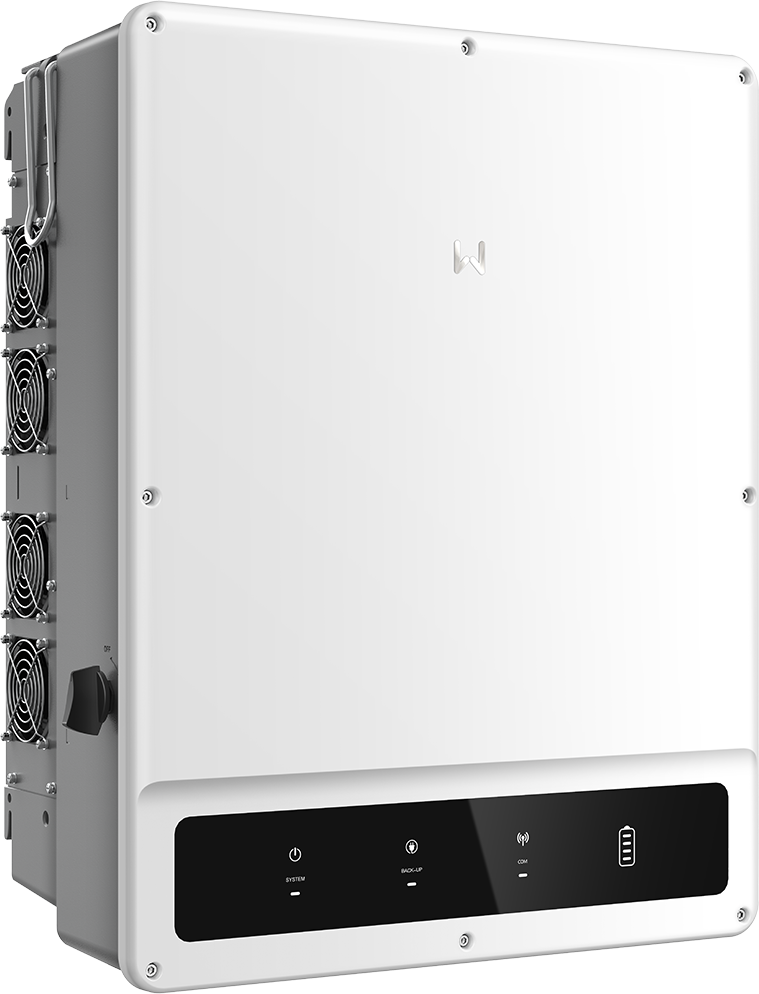
\includegraphics[height=2.6cm]{estaticas/equip-inversor-trifasico.png}\hspace{0.6cm}%
  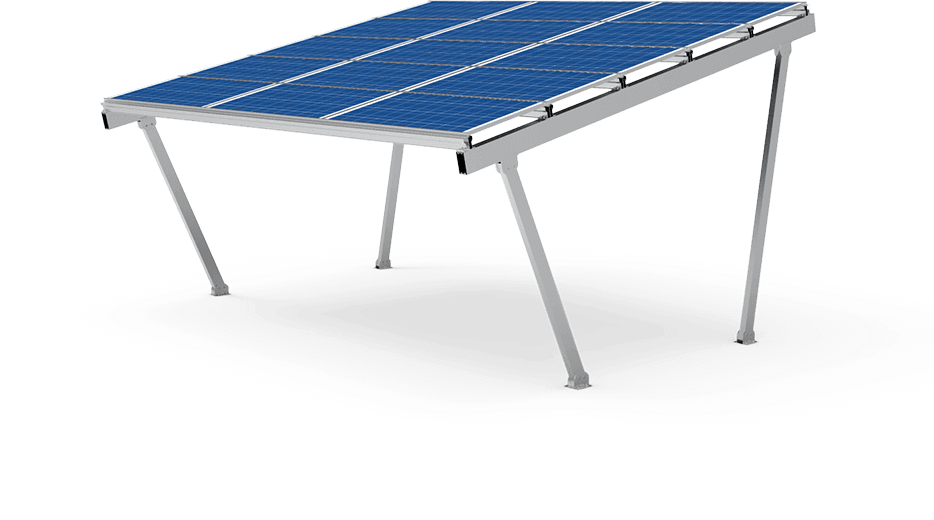
\includegraphics[height=2.6cm]{estaticas/equip-carport.png}%
}

% ---- Números institucionais (slide do monitoramento) -----------------------
\newcommand{\clientesgeridos}{+6.000}
\newcommand{\potenciagerida}{150 MWp}
